\documentclass{sig-alternate}
\usepackage[latin1]{inputenc}
\usepackage{graphicx}        % standard LaTeX graphics tool
\usepackage{url} 

\providecommand{\e}[1]{\ensuremath{\times 10^{#1}}}
\begin{document}
%
% --- Author Metadata here ---
\conferenceinfo{GECCO'13,} {July 6-10, 2013, Amsterdam, The Netherlands.}
    \CopyrightYear{2013}
    \crdata{TBA}
    \clubpenalty=10000
    \widowpenalty = 10000

\title{A service oriented evolutionary architecture: applications and results}
% uso consistente de may�sculas y min�sculas

%\subtitle{[Extended Abstract]
%\titlenote{A full version of this paper is available as
%\textit{Author's Guide to Preparing ACM SIG Proceedings Using
%\LaTeX$2_\epsilon$\ and BibTeX} at
%\texttt{www.acm.org/eaddress.htm}}}
%
% You need the command \numberofauthors to handle the 'placement
% and alignment' of the authors beneath the title.
%
% For aesthetic reasons, we recommend 'three authors at a time'
% i.e. three 'name/affiliation blocks' be placed beneath the title.
%
% NOTE: You are NOT restricted in how many 'rows' of
% "name/affiliations" may appear. We just ask that you restrict
% the number of 'columns' to three.
%
% Because of the available 'opening page real-estate'
% we ask you to refrain from putting more than six authors
% (two rows with three columns) beneath the article title.
% More than six makes the first-page appear very cluttered indeed.
%
% Use the \alignauthor commands to handle the names
% and affiliations for an 'aesthetic maximum' of six authors.
% Add names, affiliations, addresses for
% the seventh etc. author(s) as the argument for the
% \additionalauthors command.
% These 'additional authors' will be output/set for you
% without further effort on your part as the last section in
% the body of your article BEFORE References or any Appendices.


\numberofauthors{1}
 \author{
 \alignauthor
 Pablo Garc{\'i}a-S{\'a}nchez\\
        \affaddr{Dept. of Computer Architecture}\\
        \affaddr{and Computer Technology}\\
        \affaddr{University of Granada, Spain}\\
        \email{pgarcia@atc.ugr.es}
 }

%\numberofauthors{2}
% \author{
% \alignauthor
% Anonymous\\
%        \affaddr{Lost island}\\
%        \affaddr{Unknown}\\
%        \affaddr{Pacific Ocean}\\
%        \email{jack,sawyer,hurley@lost.com}
% \alignauthor
% Anonymous\\
% \affaddr{Lost island}\\
% \affaddr{Unknown}\\
% \affaddr{Pacific Ocean}\\
% \email{lock@lost.com}
% }

%\numberofauthors{2}
% \author{
% \alignauthor
% J.J. Merelo, A.M. Mora, C. M. Fernandes\\
%        \affaddr{University of Granada}\\
%        \affaddr{Department of Computer Architecture and Technology, ETSIIT}\\
%        \affaddr{18071 - Granada}\\
%        \email{jmerelo,amorag,cfernandes@geneura.ugr.es}
% \alignauthor
% Anna I. Esparcia-Alcázar\\
% \affaddr{S2 Grupo}\\
% \email{aesparcia@s2grupo.es}
% }


%\numberofauthors{4} %  in this sample file, there are a *total*
% of EIGHT authors. SIX appear on the 'first-page' (for formatting
% reasons) and the remaining two appear in the \additionalauthors section.
%

%\author{
% You can go ahead and credit any number of authors here,
% e.g. one 'row of three' or two rows (consisting of one row of three
% and a second row of one, two or three).
%
% The command \alignauthor (no curly braces needed) should
% precede each author name, affiliation/snail-mail address and
% e-mail address. Additionally, tag each line of
% affiliation/address with \affaddr, and tag the
% e-mail address with \email.
%
% 1st. author
%\alignauthor
%Jack\\
%       \affaddr{Lost island}\\
%       \affaddr{unknow}\\
%       \affaddr{Pacific Ocean}\\
%       \email{jack_the_doctor@lost.com}
% 2nd. author
%\alignauthor
%Sawyer\\
%       \affaddr{Lost island}\\
%       \affaddr{unknow}\\
%       \affaddr{Pacific Ocean}\\
%       \email{sawyer_tom@lost.com}
% 3rd. author
%\alignauthor 
%Lock\\
%       \affaddr{Lost island}\\
%       \affaddr{unknow}\\
%       \affaddr{Pacific Ocean}\\
%       \email{lock@lost.com}
% 4rd. author
%\alignauthor 
%Hurley\\
%       \affaddr{Lost island}\\
%       \affaddr{unknow}\\
%       \affaddr{Pacific Ocean}\\
%       \email{hugo@lost.com}
%}

%\and  % use '\and' if you need 'another row' of author names
% 4th. author
%\alignauthor Lawrence P. Leipuner\\
%       \affaddr{Brookhaven Laboratories}\\
%       \affaddr{Brookhaven National Lab}\\
%       \affaddr{P.O. Box 5000}\\
%       \email{lleipuner@researchlabs.org}
% 5th. author
%\alignauthor Sean Fogarty\\
%       \affaddr{NASA Ames Research Center}\\
%       \affaddr{Moffett Field}\\
%       \affaddr{California 94035}\\
%       \email{fogartys@amesres.org}
% 6th. author
%\alignauthor Charles Palmer\\
%       \affaddr{Palmer Research Laboratories}\\
%       \affaddr{8600 Datapoint Drive}\\
%       \affaddr{San Antonio, Texas 78229}\\
%       \email{cpalmer@prl.com}
%}
% There's nothing stopping you putting the seventh, eighth, etc.
% author on the opening page (as the 'third row') but we ask,
% for aesthetic reasons that you place these 'additional authors'
% in the \additional authors block, viz.
%\additionalauthors{Additional authors: John Smith (The Th{\o}rv{\"a}ld Group,
%email: {\texttt{jsmith@affiliation.org}}) and Julius P.~Kumquat
%(The Kumquat Consortium, email: {\texttt{jpkumquat@consortium.net}}).}
%\date{30 July 1999}
% Just remember to make sure that the TOTAL number of authors
% is the number that will appear on the first page PLUS the
% number that will appear in the \additionalauthors section.

\maketitle

\begin{abstract} %Se supone que ya est� desarrollado, no diga el estado de desarrollo. Di que funcionalidades tiene - JJ - FERGU: Al ser student workshop deber�a orientarlo al desarrollo de mi tesis
This paper shows the stage of development of a Service Oriented
Architecture for Evolutionary Algorithms and the first results
obtained in two different areas. %PEDRO: casi que quitar�a desde los dos puntos hasta este punto y seguido, ya que en la �ltima frase vuelves a decir esto mismo pero un poco con m�s detalle. FERGU: Done
The abstract architecture is presented, with its assocciated %"an"
                                %o "the" - JJ - FERGU The mejor
implementation using a widely used technology. Results attained in  % PEDRO: repites "results attained" en dos frases seguidas... FERGU: Pongo "obtained"
experiments with parameter adaptation in distributed heterogeneous
machines are presented and the usage of the architecture in
Evolutionary Art is also applied. 
\end{abstract}

% A category with the (minimum) three required fields
\category{H.4}{Information Systems Applications}{Miscellaneous}
%A category including the fourth, optional field follows...
\category{G.1.6}{Mathematics of Computing}{NUMERICAL ANALYSIS}[Optimization]


%sures, performance measures
\terms{Algorithms}


\keywords{Service oriented architecture, framework, parameter setting, distributed algorithms, island model, evolutionary art}


%
%%%%%%%%%%%%%%%%%%%%%%%%%%%%%%%   INTRODUCTION   %%%%%%%%%%%%%%%%%%%%%%%%%%%%%%%
%
\section{Introduction}
\label{sec:intro}
%
Ian Foster defined in \cite{SERVICEORIENTEDSCIENCE05}  the term {\em Service-Oriented Science}, that is, scientific research using interoperable and distributed networks of services, being the key of success the uniformity of interfaces, so researchers can discover and access to services without developing specific code for each data source, program or sensor. Therefore, this paradigm has the potential to increase scientific productivity thanks to the wide set of available distributed tools, and also increasing the automation of computation data analysis. On the other way, other trends such as Cloud Computing \cite{CLOUD} or GRID \cite{GRID1} are leading to heterogeneous computational devices working at the same time.  Moreover, many laboratories do not count with classic clusters, but the usual workstations used by scientists can behave in group as an heterogeneous cluster. 

Nowadays, there are many frameworks for Evolutionary Algorithms (EAs), but all of them are Object Oriented statically programmed, not taking the advantages that Service Oriented Computing is able to offer. As services must be well-defined, encapsulated and reusable, it is necessary to abstract enough to have a good EA design. In \cite{GENERICITY05} authors discuss about genericity in evolutionary computation software tools. Although their discussion is based in Object Oriented programming, the genericity of an EA framework can be applied to develop EC services, and extended with new functionalities.

Our previous work \cite{OSGILIATH} presents an abstract Service Oriented Architecture for Evolutionary Algorithms (SOA-EA), describing the set of guidelines and steps to migrate from traditional development to SOA. It also presents a specific implementation, called OSGiLiath: an environment for the development of distributed algorithms, extensible via plug-ins architecture, and based on a wide-accepted software specification (OSGi: Open Services Gateway Initiative \cite{OSGI}). %OSGi features (service-oriented architecture, declarative services, dynamic life-cycle management, or package abstraction) are used to create algorithms in a layered way. Moreover, it uses the new OSGi 4.2 distribution capabilities to develop distributed services.


%Heterogeneous dEAs can be divided in two categories: a dEA where the parameters are different in each island (heterogeneous parameters) or the same algorithm in heterogeneous hardware. It also have been proved that this kind of algorithms are even more efficient in heterogeneous hardware configurations, than in homogeneous devices \cite{HETEROGENEOUSHARD}. This can be explained by different reasons, such as different memory access times, cache, or even implementation languages or compilers in each machine, leading to different explotation rate of the search space. The heterogeneous parameters configuration also have been proved as more efficient than a fixed set of parameters for different problems \cite{HETEROGENEOUSPARAMETERS}. Our motivation in this work is to combine both ideas adapting the population size of the islands to the heterogeneous hardware. To calculate the computational power, the algorithm is executed in each machine, and then, the total size of individuals is distributed according the number of generations attained in each node during the same time. Two different problems (MMDP and OneMax) have been used as a benchmark.

This paper shows how this implementation has been used to obtain results in two different areas: one in the algorithmic scope (parameter tuning in heterogeneous devices \cite{HETEROGENEOUSHARD}) and also in the application of EAs (Evolutionary Art \cite{EVOART}).



The rest of the work is structured as follows: after the state of
the art, we present the developed service oriented architecture in Section \ref{sec:soaea}. 
Then, the results of the first experiment in heterogeneous clusters are shown (Section \ref{sec:heterogeneous}), followed by an application in Evolutionary Art (Section \ref{sec:evoart}). % PEDRO: esta referencia sale rota en el PDF FERGU: Arreglado
Finally conclusions and future lines of work are shown.


%%%%%%%%%%%%%%%%%%%%%%%%%%%%%%  SOA  %%%%%%%%%%%%%%%%%%%%%%%%%%%%%%
%
\section{State of the art}
\label{sec:soa}

Even as Service Oriented Architecture is extensively used  in software development, it is not widely extended in the EAs software scope. 
Firstly, there exist
Object Oriented frameworks, such as Al\-go\-rithm::Evo\-lu\-tionary,
JCLEC or jMetal.
 Users implement specific interfaces of these frameworks (such as {\em
   individual} or {\em crossover}) and they group them in the source
 code. For example, creating an operator object that groups several
 operators. However, these frameworks are not compatible between them.
 For example, the operators created in JCLEC can not be used in jMetal
 (despite both are programmed in Java). Also, they can not control the
 services (operators) outside the source code. Parallelism and distribution are added in other frameworks, such as
MALLBA, DREAM or ECJ, but
using external libraries (such as MPI or DRM), so the code that uses these
libraries is mixed with the algorithm's code.



Even being distributed, these frameworks can not communicate with each other. HeuristicLab is one of the few plug-in and service oriented frameworks. It uses web services for communication, but just to distribute the load, after consulting a central database of available jobs. The work \cite{SURVEYMOFS} contains a comparison and the references of the previous frameworks. %Finally, the only service oriented optimization framework is GridUFO \cite{GRIDUFO}, but it only allows the modification of the objective function and the addition of whole algorithms, without combining existing services.
%

%In the field of the Evolutionary Computing there are two different approaches about the algorithm parameter setting: parameter control and parameter tuning \cite{PARAMETERTUNING}. The first one refers to set a number of parameters of an EA and to change these parameter while the algorithm is running. The parameter tuning consist in establish a good set of parameters before the run (and do not change them during runtime).

%Computational performance of nodes or network speeds can also be inherents parameter of an algorithm. In \cite{HETEROGENEOUSHARD} authors compared a distributed GA in homogeneous and heterogeneous clusters. Super-linear performance was obtained in the heterogeneous clusters, being more efficient that the same algorithm in homogeneous ones. Some authors have expanded this idea adapting the algorithm to be executed: in \cite{HYDROCM} authors presented a distributed hybrid meta-heuristic that combines GAs and Simulated Annealing (SA). Their system executes the costly algorithms (GAs) in faster nodes, and simpler meta-heuristics (SA) in slower nodes, obtaining better results than other configurations. In \cite{HETEROGENEOUSTOPOLOGY} different configurations of heterogeneous machines for a tree topology were studied. However, the heterogeneity was simulated in an homogeneous clusters with programs to add computational load. Load-balancing was also applied taking into account the computational load of the nodes in \cite{PARALLELIMPLEMENTATION}: a small benchmark was executed in all nodes at the beginning of the algorithm to distribute individuals of an Evolutionary Strategy (ES). However, there was not communication between the nodes. In the area of heterogeneous parameters, but homogeneous hardware, setting each island a random set of parameters can also increase the performance of a distributed Genetic Algorithm (dGA), as explained in \cite{HETEROGENEOUSPARAMETERS}. That model outperformed a tuned canonical dGA with the same parameters in all islands. Finally, adapting the migration period has produced better results than homogeneous periods in homogeneous clusters, as explained by \cite{HETEROGENEOUSMIGRATION}.

%Our work presents a combination of previous ideas, where a parameter
%tuning given by the computational cost of the machines is
%performed. For our knowledge, there are not works that modify
%parameters of the GA depending of the node where the island is being
%executed.

% Habla tambi�n del Algorithm::Evolutionary, hombre... - JJ -FERGU: Si lo he mencionao arriba!

Other field related is the heterogeneous evolutionary computing, where two areas exist: heterogeneous hardware and heterogeneous parameters. In the first area  authors study or adapt algorithms depending on the machine configuration \cite{HETEROGENEOUSHARD, HETEROGENEOUSTOPOLOGY}. In the area of heterogeneous parameters,  setting in each island (node) a different sets of parameters can also increase the performance of distributed EAs, as explained in \cite{HETEROGENEOUSPARAMETERS, HETEROGENEOUSMIGRATION}.

Our work presents a combination of these ideas, where a parameter tuning given by the computational power of the machines is performed. To our knowledge, there are not works that modify parameters of the EA depending of the node where the island is being executed.

%%%%%%%%%%%%%%%%%%  Experiments  %%%%%%%%%%%%%%%%%%%
\section{A Service Oriented Architecture for Evolutionary Algorithms}
\label{sec:soaea}

In \cite{OSGILIATH} we presented an abstract architecture composed by loosely coupled, highly configurable and
lan\-gua\-ge-in\-de\-pen\-dent services for Evolutionary Computation (called SOA-EA). As example of implementation 
of this architecture, a complete process development using a specific service oriented 
technology (OSGi) was explained. With this implementation, less effort than classical development 
in integration, distribution mechanisms and execution time management has been attained. 
In addition, steps, ideas, advantages and disadvantages, and guidelines to create service oriented
evolutionary algorithms were explained.

In \cite{GENERICITY05}, six criteria for qualify EA frameworks were presented: generic representation, fitness, operator, model, parameters management and configurable output. In our previous work we shown how SOA follows these lines of genericity, but can also extend them:
\begin{itemize}
\item Genericity in the service interfaces: service interfaces are established to create new implementations. Furthermore, these interfaces must be abstract enough to avoid their modification.
\item Programming language independence: for example, services implemented in Java can use services implemented in C++ and vice-versa.
\item Distribution transparency: it is not mandatory to use a specific library for the distribution, or modify the code to adapt the existing operators.
\item Flexibility: easy to add and remove elements to use the self-adaptation or other mechanisms.
\end{itemize}

A specific implementation of our architecture (called OSGiLiath) has been developed using the OSGi service oriented technology, with a number of services already developed. These services can be combined in several ways to obtain different algorithms, and can be dynamically bound to cha\-nge the needed EA features. In addition, new services can be added in execution time using our implementation. No specific source code for a basic distribution needs to be added, neither the existing source code has been modified to achieve the previous tasks.


\section{Adapting the population size to hardware}
\label{sec:heterogeneous}

One of the first experiments performed with OSGiLiath has been to establish the effect of the population size in homogeneous and heterogeneous clusters. 
The algorithm to be improved is a distributed Genetic Algorithm. The algorithm is steady-state: the offspring is mixed with the parents and the worst individuals are removed. A ring topology is used, and the best individual is sent after a fixed number of generations of each node (64).  Two different parameter configurations have been used: 64 individuals per node (homogeneous size) and a different number of individuals proportional to the computational power of each node. An uniform crossover is used (with a rate of 0.5) and a bit-flip mutation (with a probability of 1/genome size).


The problems to evaluate are the Massively Multimodal Deceptive Problem (MMDP) \cite{goldberg92massive} and the OneMax problem \cite{ONEMAX}. Each one requires different actions/abilities by the GA at the level of population sizing, individual selection and building-blocks mixing. The chromosome length is 150 for MMDP and 5000 for OneMax. %The MMDP  is designed to be difficult for an EA, due to its multimodality and deceptiveness. Deceptive problems are functions where low-order building-blocks do not combine to form higher order building-blocks. Instead, low-order building-blocks may mislead the search towards local optima, thus challenging search mechanisms. MMDP it is composed of $k$ subproblems of 6 bits each one ($s_i$). Depending of the number of ones (unitation) $s_i$ takes the values shown in Table \ref{table:mmdp}.  




%The fitness value is defined as the sum of the $s_i$ subproblems with an optimum of $k$ (equation \ref{eq:mmdp}).
%The search space is composed of $2^{6k}$ combinations from which there
%are only $2^k$ global solutions with $22^k$ deceptive
%attractors. Hence, a search method will have to find a global solution
%out of $2^{5k}$ additionally to deceptiveness. In this work $k=25$. 


%OneMax is a simple linear problem that consists in maximising the number of ones in a binary string.


To test the algorithm two different computational systems have been used: an {\em heterogeneous cluster} and an {\em homogeneous cluster}. The first one is formed by 4 different computers of our lab with different processors, operating systems and memory size. The latter is a dedicated scientific cluster formed by homogeneous nodes. Table \ref{tab:computers} shows the features of each system.

\begin{table*}
\centering{\scriptsize
\caption{Details of the clusters used.}
\begin{tabular}{|c|c|c|c|c|} \hline
Name 		 & Processor 	& Memory 	& Operating System  & Network  \\ \hline
\multicolumn{5}{|c|}{Homogeneous cluster} \\ \hline
Cluster node &	Intel(R) Xeon(R) CPU   E5320  @ 1.86GHz		    &	4GB	& CentOS 6.7		& 	Gigabit Ethernet  	\\ \hline
\hline
\multicolumn{5}{|c|}{Heterogeneous cluster} \\ \hline
N1	&	 Intel(R) Core(TM)2 Quad CPU    Q6600  @ 2.40GHz		& 4GB		&	Ubuntu 11.10 (64 bits)	&	Gigabit Ethernet	  	\\ \hline
N2 	&	 Intel(R) Core(TM)2 Quad CPU    Q6600  @ 2.40GHz		& 4GB		&	Ubuntu 11.04 (64 bits)	&	Gigabit Ethernet	  	\\ \hline
N3 	&	 AMD Phenom(tm) 9950 Quad-Core Processor @ 1.30Ghz		& 3GB		&	Ubuntu 10.10 (32 bits)	&	100MB Ethernet	  	\\ \hline
N4 	&	 Intel (R) Pentium 3 @ 800MHz		    				& 768 MB	&	Ubuntu 10.10 (32 bits)	& 	10MB Ethernet	  	\\ \hline
\end{tabular}
}
\label{tab:computers}
\end{table*}

%Because the operating system and architecture heterogeneity the ANONYMOUS framework \cite{OSGILIATH}, based in Java, has been used. This is a service-oriented evolutionary framework that automatically configures services to use and be used in a local network. In this case, each node offers a migration buffer to accept foreign individuals. Also, to avoid bottlenecks in distributed executions, asynchronous communication has been provided to avoid idle time using reception buffers (that is, the algorithm does not wait until new individuals arrive). This kind of communication offers excellent performance when working with different nodes and operating systems, as demonstrated by \cite{HETEROGENEOUSHARD}. The transmission mechanism is based in ECF Generic server (over TCP)\footnote{\url{http://www.eclipse.org/ecf/}}. The source code of the algorithms used in this work is available in \url{http://anonymous} under a GPL V3 License.

Acronyms for each configuration are HoSi (homogeneous population size), HeSi (heterogeneous population size), HoHa (homogeneous hardware) and HeHa (heterogeneous hardware). 

Each different configuration has been tested 30 times. The number of individuals in each node of the HeSi configuration is proportional the computational power of each node. In this case the computational power has been calculated comparing the average number of generations obtained in the nodes of the HoSi/HeHa configuration for the MMDP problem. Thus, the HeSi configuration uses 98, 84, 66, and 8 individuals (from N1 to N4). Note that, having two nodes with the same processors and memory (N1 and N2), they have different computational power.
%%%%%%%%%%%%%%%%%%  Results  %%%%%%%%%%%%%%%%%%%

\subsection{Results}

The objectives of the parallel programming are to tackle large computational problems, increase the performance of algorithms in a finite time, or reduce time. In this work we focus in the last objective. As claimed by \cite{EVALUATIONPARALLEL}, the number of evaluations can be misleading in the parallel algorithms area. In our case, for example, the evaluation time is different in each node of the heterogeneous cluster, and the real algorithm speed could not be reflected correctly. However, the number of evaluations has been added in this section to better understand the results. Also, the total number of generations, and the maximum number of generations of the slower node are shown. It is difficult to compare between  HoHa and HeHa for the same reason: the evaluation time is different in each system (and also in each node).

% Pero tienes que hacer �nfasis en lo f�cil que ha sido desarrollarlo
% y sacar resultados nuevos y todo eso - JJ. FERGU: es que eso va para el del EvoSoft xD

\subsubsection{MMDP Problem}
Table \ref{tab:resultsMMDP} shows the results for the MMDP problem.  In the HeHa system, adapting the population to the computational power of each node makes the algorithm to end significantly faster, but with the same number of evaluations (with no statistical significance). This can be explained because the evaluation time is different in all nodes. On the other hand, in the HoHa system, setting the same population sizes makes no difference in time and evaluations, that is, changing this parameter does not influence the performance of the algorithm (no statistically significance attained).  %First, a Kolmogorov-Smirnov test is performed to asset the normality of the distributions. If the results fit a normal distribution, then a Student's T-Test is calculated. Otherwise, the non-parametric test Wilcoxon signed rank is applied.



\begin{table*}
\centering
\caption{Results for the MMDP problem.}
\begin{tabular}{|c|c|c|c|c|} \hline
Configuration	& Max. generations			& Total generations			& 	Total evaluations			& Time (ms) \\ \hline
HoSi/HeHa		& 146401,48	$\pm$ 65699,69	& 380967,25	$\pm$ 168568,84	& 24382416,51 $\pm$	10788405,87	& 136914,03 $\pm$ 60028,48\\ \hline
HeSi/HeHa		& 96051,5	$\pm$ 45110,90	& 289282,3	$\pm$ 135038,10	& 21784528,66 $\pm$	10161989,38	& 109875,76 $\pm$ 49185,51\\ \hline \hline
HoSi/HoHa		& 107334,46 $\pm$ 78167,19  & 393119,86 $\pm$ 241835,27	& 25273201,06 $\pm$ 15386663,12	& 237759,43 $\pm$ 178709,86\\ \hline
HeSi/HoHa		& 149732,6 $\pm$ 81983,74	& 438171,16	$\pm$ 240169,19	& 24430043,46 $\pm$ 13395037,34	& 245776,93 $\pm$ 134715,52\\ \hline

\end{tabular}
\label{tab:resultsMMDP}
\end{table*}
%%%%CAMBIAR EL ORDEN!!!

%MMDP EVALS
%HomoSizeHomoHard-HomoSizeHeteroHard 22.83333     23.69541      FALSE
%HomoSizeHomoHard-HeteroSizeHomoHard  4.90000     23.69541      FALSE
%HomoSizeHomoHard-HeteroSizeHeteroHard 37.53333     23.69541       TRUE
%HomoSizeHeteroHard-HeteroSizeHomoHard 27.73333     23.69541       TRUE
%HomoSizeHeteroHard-HeteroSizeHeteroHard 14.70000     23.69541      FALSE
%HeteroSizeHomoHard-HeteroSizeHeteroHard 42.43333     23.69541       TRUE





%\begin{figure}
%\centering
%\epsfig{file=images/timeMMDP.eps, width = 7cm}
%\caption{Time to obtain the optimum in the MMDP problem (milliseconds). White is the heterogeneous cluster and gray the homogeneous one.}
%\label{fig:timeMMDP}
%\end{figure}



%To see the difference of how the evolution is being performed, the average fitness in each node of HeHa is shown in Figures \ref{fig:hosiheha} and \ref{fig:hesiheha}. As can be seen, with the HeSi (Figure \ref{fig:hesiheha}), the local optima are overtaken in less time than HoSi (Figure \ref{fig:hosiheha}).  This can be explained because in HeSi, the migration from N4 to N1 is performed faster, adding more heterogeneity to the whole system. White gaps in the figures are the time where the nodes are sending the individual to other nodes (not while they are receiving them). In the HoHa systems, the populations are evolved at the same time, being the average fitness similar in all nodes during all run. % The natural migration period variation from a processor to another is also giving more diversity to the populations that migrating at the same time of the homogeneous




\subsubsection{OneMax Problem}

Results for OneMax are shown in Table \ref{tab:onemaxresults}. In this problem, adapting the population sizes decreases significantly the time for solving in the heterogeneous cluster, and, as before, the number of evaluations remains the same. In the homogeneous system, the effect of changing the population sizes is more evident, and this time the evaluations (and therefore, the time) are reduced (both significantly). 

The efficiency on OneMax problems depends more on the ability to mix the building-blocks, and less on the genetic diversity and size of the population (as with MMDP). No genetic diversity is particularly required. When properly tuned, a simple Genetic Algorithm is able to solve OneMax in linear time. Sometimes, problems like OneMax are used as control functions, in order to check if very efficient algorithms on hard functions fail on easier functions. %As can be seen in Figure \ref{fig:gensonemaxhomosize}, the HoSi/HeHa, the average fitness of all populations are increasing in linear way. However, the lower processor evaluates extremely less times.  On the other side, in Figure \ref{fig:gensonemaxheterosize}, the adaptation of the population size makes that lower processors increase the number of evaluations, but the average fitness is also maintained in linear way (and in smaller increase rate) between migrations. However, the other processors are still spending more number of evaluations. That is the reason why the number of evaluations is higher in HeHa, and lower in HoHa. Computational time is more efficiently used in faster nodes, having more chance to mix the individuals. Also, because the larger size of the individuals in the OneMax problem (5000 bits vs. 150), the transmission time is larger, (white gaps in the figures). That also implies for N4 send their best individual to N1 in a extremely large time when using HoSi (each 64 generations).

\begin{table*}
\centering
\caption{Results for the OneMax problem.}
\begin{tabular}{|c|c|c|c|c|} \hline
Configuration	& Max. generations			& Total generations			& 	Total evaluations			& Time (ms) \\ \hline
HoSi/HeHa		& 4739,41$\pm$	305,32 		&	12081,51$\pm$	776,35 	&	773729,03$\pm$	49686,72 	&	72152,32$\pm$	4994,71 \\ \hline
HeSi/HeHa		&	3438,03 $\pm$	149,47 &	11277,33$\pm$	471,77 &	794157,73$\pm$	31843,10 	&	61870,2	$\pm$ 2518,74 \\ \hline \hline
HoSi/HoHa		&	3133,36$\pm$	101,70 	&	12347,83$\pm$	394,99 	&	790773,33$\pm$	25279,52 	&	62105,03$\pm$	1964,75 \\ \hline
HeSi/HoHa		& 13897,86$\pm$	625,27 		&	20725,63$\pm$	929,43 	&	651952,8 $\pm$	29114,54	&	56120,53$\pm$	2491,92 \\ \hline
\end{tabular}
\label{tab:onemaxresults}
\end{table*}



%\begin{figure}
%\centering
%\epsfig{file=images/timeOneMax.eps, width = 7cm}
%\caption{Time to obtain the optimum in the OneMax problem (milliseconds). White is the heterogeneous cluster and gray the homogeneous one.}
%\label{fig:timeOneMax}
%\end{figure}




%\begin{table}
%\centering
%\caption{Frequency of Special Characters}
%\begin{tabular}{|c|c|l|} \hline
%Non-English or Math&Frequency&Comments\\ \hline
%\O & 1 in 1,000& For Swedish names\\ \hline
%$\pi$ & 1 in 5& Common in math\\ \hline
%\$ & 4 in 5 & Used in business\\ \hline
%$\Psi^2_1$ & 1 in 40,000& Unexplained usage\\
%\hline\end{tabular}
%\end{table}


%\begin{figure}
%\centering
%\epsfig{file=fly.eps}
%\caption{A sample black and white graphic (.eps format).}
%\end{figure}
%
%\begin{figure}
%\centering
%\epsfig{file=fly.eps, height=1in, width=1in}
%\caption{A sample black and white graphic (.eps format)
%that has been resized with the \texttt{epsfig} command.}
%\end{figure}

%\begin{figure*}
%\centering
%\epsfig{file=flies.eps}
%\caption{A sample black and white graphic (.eps format)
%that needs to span two columns of text.}
%\end{figure*}

\section{Comparing his\-to\-grams in Evolutionary Art}
\label{sec:evoart}

OSGiLiath has also been used to study the differences of
using the information of the HSV (Hue, Saturation, Value) and
RGB (Red, Green, Blue) histograms during the evolution of an aesthetical image. A service to access to Processing
\cite{PROCESSING}, a programming framework designed for visual artists, have been performed. In addition, services to measure the fitness, and implementations of individuals are also available in OSGiLiath. Processing is used inside
the EA to model the individuals,
generate their associate images and extract information of
them (HSV, RGB and Average histograms) to fit with the
histograms of a test image. 

A steady-state evolutionary algorithm has been used. Each individual is randomly generated at the initialization of the EA. The genome size is 50 elements (circles of maximum radium of 128 pixels). Population size has been set to 32 individuals. Uniform crossover rate is 0.5, and a binary tournament has been chosen for selection. Mutation probability is 0.04 (the usual value of {\em 1/genomesize}). Finally, the image size for each individual is 256x256 pixels. The individuals have been compared with the histograms obtained from an aesthetic predefined image to guide the evolution.

Three different fitness functions using color histogram have been tested and added to OSGiLiath as services: difference between the HSV and RGB histograms, and an average difference of the two histograms at the same time. Table \ref{tab:artresults} show the attained results. Experiments show that better results in terms of similarity are obtained using the HSV comparison (due to the noisy information provided by the RGB). This is a basic image metric, only used by purposes of proof-of-concept and more complex measurements will be studied in future works. % PEDRO: he cambiado next por future. FERGU: Guay



\begin{table}
\centering
\caption{Results for the different fitness. Only one histogram type is used, but the other values obtained are also added.}
\resizebox{8cm}{!}{
\begin{tabular}{|c|c|c|c|} \hline
Differences used & Obtained RGB      		& Obtained HSV  & Obtained Average \\ \hline
RGB     & {\em 0.267 $\pm$ 0.012}	& 0.170 $\pm$ 0.010 	& 0.218 $\pm$ 0.009	\\ \hline
HSV     & 0.227 $\pm$ 0.017	& {\em 0.265 $\pm$ 0.021}	& 0.246 $\pm$ 0.010 \\ \hline
Average & 0.173 $\pm$ 0.012	& 0.294 $\pm$ 0.013	& {\em 0.234 $\pm$ 0.010} \\ \hline
\end{tabular}
}
\label{tab:artresults}
\end{table}

% �Alg�n experimento espec�fico que puedas desarrollar r�pidamente?  JJ Fergu: puf, a ver si hago algo.

\section{Conclusions}
Service Oriented Computing is a new trend where computational resources cooperate in an automatic way without taking into account programming language or operating system. 
Also, other trends, such as Cloud Computing are providing a massively amount of heterogeneous computational devices. This has been the motivation to develop SOA-EA and OSGiLiath.

The first applications have been a preliminary study about adapting the population size of an EA to computational power of different nodes in an heterogeneous cluster. Results show that adapting the population size decrease the execution time significantly in heterogeneous clusters, while changing this parameter in homogeneous clusters not always performs better. This is a promising start for adapting EAs to the computational power of each execution node.

As future work a scalability study will be performed, with more computational nodes and larger problem instances. Moreover, other parameters such as migration rate or crossover probability will be adapted to the execution nodes. This studies will lead to automatic adaptation during runtime, with different nodes entering or exiting in the topology during the algorithm execution or adapting to the current load of the system.

Finally, new experiments in the field of Evolutionary Art will be performed.

The project development is explained and also avaible for download and modification under a GPL V3 License at \url{http://www.osgiliath.org}


%ACKNOWLEDGMENTS are optional
\section{Acknowledgments}
This work has been supported in part by FPU research grant AP2009-2942 and projects EvOrq (P08-TIC-03903), UGR PR-PP2011-5 and TIN2011-28627-C04-02.

%
% The following two commands are all you need in the
% initial runs of your .tex file to
% produce the bibliography for the citations in your paper.


%\bibliographystyle{abbrv} CAMBIAR!!!!!!
\bibliographystyle{plain}
\bibliography{soahetero}  % sigproc.bib is the name of the Bibliography in this case


\end{document}
